%% Copyright (c) 2015-2019, RTE (http://www.rte-france.com)
%% See AUTHORS.txt
%% All rights reserved.
%% This Source Code Form is subject to the terms of the Mozilla Public
%% License, v. 2.0. If a copy of the MPL was not distributed with this
%% file, You can obtain one at http://mozilla.org/MPL/2.0/.
%% SPDX-License-Identifier: MPL-2.0

%% This file is part of Dynawo, an hybrid C++/Modelica open source time domain
%% simulation tool for power systems.

\documentclass[a4paper, 12pt]{report}
\usepackage{graphicx}
\usepackage{float}

\usepackage{xspace}
\usepackage{tikz}
\usepackage{array}
\usepackage{pgfplots} %for graphics
\pgfplotsset{compat=newest}
\usetikzlibrary[pgfplots.groupplots]
\usepgfplotslibrary{groupplots}
\usetikzlibrary{matrix,arrows,decorations.pathmorphing}
\definecolor{myblue}{rgb}{0.0,0.57,0.81}
\definecolor{myred}{rgb}{0.86,0,0.17}
\definecolor{mygreen}{rgb}{0,0.58,0}
\definecolor{mygray}{rgb}{0.4,0.4,0.4}
\definecolor{myyellow}{rgb}{1,0.84,0.024}
\definecolor{mycyan}{rgb}{0.19,0.835,0.87}
\definecolor{mypurple}{rgb}{0.635,0.055,0.67}
\definecolor{myorange}{rgb}{0.86,0.44,0.145}
\definecolor{myblueT}{rgb}{0.082,0.48,0.76}
\definecolor{myredT}{rgb}{0.84,0.18,0.18}

\newcommand{\Dynawo}[0]{Dyna$\omega$o\xspace}
 
\tikzset{generator1/.pic={
        code={
        	\draw (0,0) circle (2);
            \draw (0,0) arc (0:180:0.5);
            \draw (0,0) arc (180:360:0.5);
            \draw (2,0) --++ (2,0);
 	}
  }
}

\tikzset{generator2/.pic={
        code={
        	\draw (0,0) circle (2);
            \draw (0,0) arc (0:180:0.5);
            \draw (0,0) arc (180:360:0.5);
            \draw (-2,0) --++ (-2,0);
 	}
  }
}

\tikzset{transfo/.pic={
        code={
        \draw (0,0) circle (2);
        \draw (2,0) circle (2);
        \draw (4,0) --++ (4,0);
        \draw (-2,0) --++ (-4,0);
 	}
  }
}

\tikzset{Governor/.pic={
        code={
        \draw (0,0) circle (2) node[inner sep=0, outer sep=0] {{Gov}};
 	}
  }
}

\tikzset{Load/.pic={
        code={
        \draw (0,0) circle (2) node[inner sep=0, outer sep=0] {{Load}};
 	}
  }
}

\begin{document}

\chapter*{Test - "Small Case + Governor"}
This is the documentation for the test "Small Case + Governor" in the \Dynawo project non regression tests.

% Generic description of the non regression test
% Data origin, network size, simulation types and numbers, etc.
\section*{Test description}

This document presents a basic unit test based on a dyd file which instantiates a synchronous machine models connected through a line and a transformer to another synchronous machine and two loads, as presented in Figure 1. The first machine's mechanical power is controlled by a proportional governor. Here, we want to observe how the system reacts to the loss of one of the loads during the simulation. In the following, this test's results will be compared to the same configuration with the governor replaced by a set point on $PmPu$.

\begin{figure}[H]
\centering
\def\factor{0.4}
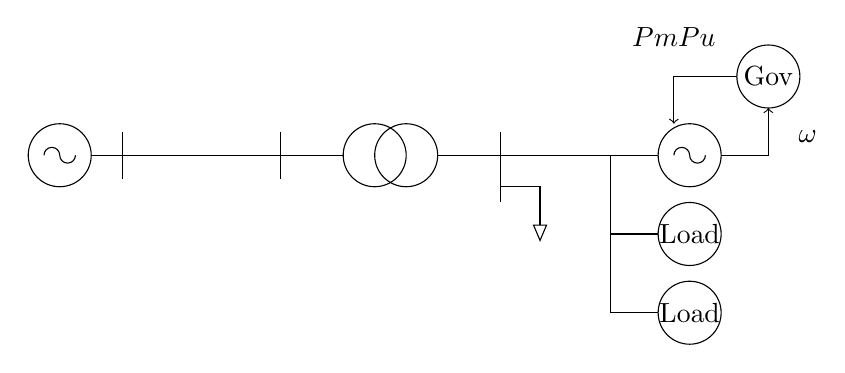
\begin{tikzpicture}[every node/.style={inner sep=0,outer sep=0}]
% Gen1
\path (0,0)  pic[scale=0.2,local bounding box=gen1] {generator1};
%% Transfo
\path (4,0) pic[scale=0.2,local bounding box=transfo] {transfo};
% Gen2
\path (8,0) pic[scale=0.2,local bounding box=gen2] {generator2};
% Governor
\path (9,1) pic[scale=0.2,local bounding box=Governor] {Governor};
% Loads
\path (8,-1) pic[scale=0.2,local bounding box=Load1] {Load};
\path (8,-2) pic[scale=0.2,local bounding box=Load2] {Load};
% Line
\draw (gen1.east) -- (transfo.west);
\draw (transfo.east) -- (gen2.west);
% Bus inf
\draw (gen1.east) ++ (0,0.3) --++ (0,-0.6);
% Bus tfo 1
\draw (transfo.west) ++ (0,0.3) node (bustop) {} --++ (0,-0.6) node (busbottom) {};
% Bus tfo 2
\draw (transfo.east) ++ (0,0.3) node (bustop) {} --++ (0,-0.9) node (busbottom) {};
% Load
\draw ([yshift=0.2cm]busbottom.center) --++ (0.5, 0) [-open triangle 45] --++ (0,-0.7);
\draw [->] (Governor.west) -| node [pos=0.5,yshift=0.5cm] {$PmPu$}(gen2.north);
\draw [->] (gen2.east) -| node [pos=0.7,xshift=0.5cm] {$\omega$} (Governor.south);
\draw (Load1.west) -| (7, 0);
\draw (Load2.west) -| (7, 0);
\end{tikzpicture}
\caption{Test case}
\label{circuit-1}
\end{figure}

\begin{figure}[H]
\centering
\def\factor{0.4}
\begin{tikzpicture}[every node/.style={inner sep=0,outer sep=0}]
% Gen1
\path (0,0)  pic[scale=0.2,local bounding box=gen1] {generator1};
%% Transfo
\path (4,0) pic[scale=0.2,local bounding box=transfo] {transfo};
% Gen2
\path (8,0) pic[scale=0.2,local bounding box=gen2] {generator2};
% Loads
\path (8,-1) pic[scale=0.2,local bounding box=Load1] {Load};
\path (8,-2) pic[scale=0.2,local bounding box=Load2] {Load};
% Line
\draw (gen1.east) -- (transfo.west);
\draw (transfo.east) -- (gen2.west);
% Bus inf
\draw (gen1.east) ++ (0,0.3) --++ (0,-0.6);
% Bus tfo 1
\draw (transfo.west) ++ (0,0.3) node (bustop) {} --++ (0,-0.6) node (busbottom) {};
% Bus tfo 2
\draw (transfo.east) ++ (0,0.3) node (bustop) {} --++ (0,-0.9) node (busbottom) {};
% Load
\draw ([yshift=0.2cm]busbottom.center) --++ (0.5, 0) [-open triangle 45] --++ (0,-0.7);
\draw [->] (9, 1) -| node [pos=0.5,xshift=2.2cm] {$PmPu_0$}(gen2.north);
\draw (Load1.west) -| (7, 0);
\draw (Load2.west) -| (7, 0);
\end{tikzpicture}
\caption{Test case without governor}
\label{circuit-1}
\end{figure}


% Description of the simulation
% Events, solver, duration, outputs, etc.
\subsection*{Simulation description}

Here are the important settings for both tests:

\begin{itemize}
\item The initial state on machine 1 is: $P_0$=380 MW, $Q_0$=0 MVar.
\item The initial state on machine 2 is: $P_0$=0.01 MW, $Q_0$=0 MVar.
\item The initial state on both loads is: $P_0$=190 MW, $Q_0$=0 MVar.
\item The generator is a four-winding generator.
\item The generator is initialized from internal parameters.
\item No transformer is included in the model.
\item We use IDA solver with the following characteristics:
$Order$=2, $Accuracy_{Rel}$=10e-6, $Accuracy_{Abs}$=10e-6.
\item The load disconnection happens at $t=30s$;
\item The simulation lasts for 80 s.
\end{itemize}



% Expected results
% Events, logs, plots, etc.
\subsection*{Expected results}


In this test, after the load disconnection, we expect:

\begin{itemize}
\item The electrical power first to drop, oscillate and then follow the mechanical power.
\item The angular velocity first to increase and then stabilize to a higher value once electric and mechanical powers are balanced.
\item The mechanical power controlled by the governor first to drop as the angular velocity surges, and then stabilize at a lower value.
\item In comparison to a case without the governor (i.e. mechanical power set to a constant), the angular velocity should be kept closer to its initial value when reacting to the load disconnection. 
\end{itemize}

The following plots illustrate the aforementioned points:

\begin{figure}[H]
  \caption{Machine 1 Pulsation (p.u)}
  \begin{tikzpicture}
    \begin{axis}[
        axis background/.style={fill=white},
        %title = {\begin{small}Synchronous machine electrical power - comparison with Eurostag (p.u)\end{small}},
        ymin = 0.99,
        ymax = 1.05,
        xmin = 0,
        xmax = 80,
        xtick= {0,10,...,80},
        ytick= {1,1.01,...,1.07},
        /pgf/number format/precision=3,
        x label style={at={(axis description cs:0.5,-0.15)},anchor=north},
        y label style={at={(axis description cs:0.,0.45)},anchor=south},
        xlabel={\begin{small}$time$ (s)\end{small}},
        height=0.6\textwidth,
        width=1\textwidth
        ]
        \addplot[color=myredT!50,no markers,line width=1pt,each nth point={1}]
        table[x=time,y=MS1_gover_omegaPu, col sep=semicolon]
        {../reference/outputs_SmallCase+Governor_2MS/curves/curves.csv};
        \legend{$\omega Pu_{Dynawo}$}
    \end{axis}
  \end{tikzpicture}
\end{figure}

\begin{figure}[H]
  \caption{Machine 1 behaviour (p.u)}
  \begin{tikzpicture}
    \begin{axis}[
        axis background/.style={fill=white},
        %title = {\begin{small}Synchronous machine electrical power - comparison with Eurostag (p.u)\end{small}},
        ymin = 0.45,
        ymax = 0.8,
        xmin = 0,
        xmax = 80,
        xtick= {0,10,...,80},
        ytick= {0.4,0.5,...,0.8},
        /pgf/number format/precision=3,
        x label style={at={(axis description cs:0.5,-0.15)},anchor=north},
        y label style={at={(axis description cs:0.,0.45)},anchor=south},
        xlabel={\begin{small}$time$ (s)\end{small}},
        height=0.6\textwidth,
        width=1\textwidth
        ]
        \addplot[color=myredT!50,no markers,line width=1pt,each nth point={1}]
        table[x=time,y=MS1_gen_PePu, col sep=semicolon]
        {../reference/outputs_SmallCase+Governor_2MS/curves/curves.csv};
        \addplot[dashed, color=myblueT!50,no markers,line width=1pt,each nth point={1}]
        table[x=time,y=MS1_gen_PmPu, col sep=semicolon]
        {../reference/outputs_SmallCase+Governor_2MS/curves/curves.csv};
        \legend{$PePu$,$PmPu$}
    \end{axis}
  \end{tikzpicture}
\end{figure}



\subsubsection*{Comparison against test case without a governor}

\begin{figure}[H]
  \caption{Machine 1 Pulsation (p.u)}
  \begin{tikzpicture}
    \begin{axis}[
        axis background/.style={fill=white},
        %title = {\begin{small}Synchronous machine electrical power - comparison with Eurostag (p.u)\end{small}},
        ymin = 0.99,
        ymax = 1.17,
        xmin = 0,
        xmax = 80,
        xtick= {0,10,...,80},
        ytick= {1,1.02,...,1.17},
        /pgf/number format/precision=3,
        x label style={at={(axis description cs:0.5,-0.15)},anchor=north},
        y label style={at={(axis description cs:0.,0.45)},anchor=south},
        xlabel={\begin{small}$time$ (s)\end{small}},
        height=0.6\textwidth,
        width=1\textwidth,
        legend pos=north west
        ]
        \addplot[color=myredT!50,no markers,line width=1pt,each nth point={1}]
        table[x=time,y=MS1_gen_omegaPu, col sep=semicolon]
        {../reference/outputs_SmallCase+Governor_2MS/curves/curves.csv};
        \addplot[dashed, color=myblueT!50,no markers,line width=1pt,each nth point={1}]
        table[x=time,y=MS1_gen_omegaPu, col sep=semicolon]
        {../reference/outputs_SmallCase_2MS/curves/curves.csv};
        \legend{$\omega Pu_{Governor}$,$\omega Pu_{NoGovernor}$}
    \end{axis}
  \end{tikzpicture}
\end{figure}

\begin{figure}[H]
  \caption{Machine 1 behaviour (p.u)}
  \begin{tikzpicture}
    \begin{axis}[
        axis background/.style={fill=white},
        %title = {\begin{small}Synchronous machine electrical power - comparison with Eurostag (p.u)\end{small}},
        ymin = 0.45,
        ymax = 0.8,
        xmin = 0,
        xmax = 80,
        xtick= {0,10,...,80},
        ytick= {0.4,0.5,...,0.8},
        /pgf/number format/precision=3,
        x label style={at={(axis description cs:0.5,-0.15)},anchor=north},
        y label style={at={(axis description cs:0.,0.45)},anchor=south},
        xlabel={\begin{small}$time$ (s)\end{small}},
        height=0.6\textwidth,
        width=1\textwidth,
        legend pos=south east
        ]
        \addplot[color=myredT!50,no markers,line width=1pt,each nth point={1}]
        table[x=time,y=MS1_gen_PePu, col sep=semicolon]
        {../reference/outputs_SmallCase+Governor_2MS/curves/curves.csv};
        \addplot[color=myorange!50,no markers,line width=1pt,each nth point={1}]
        table[x=time,y=MS1_gen_PePu, col sep=semicolon]
        {../reference/outputs_SmallCase_2MS/curves/curves.csv};
        \addplot[dashed, color=myblueT!50,no markers,line width=1pt,each nth point={1}]
        table[x=time,y=MS1_gen_PmPu, col sep=semicolon]
        {../reference/outputs_SmallCase+Governor_2MS/curves/curves.csv};
        \addplot[dashed, color=mypurple!50,no markers,line width=1pt,each nth point={1}]
        table[x=time,y=MS1_gen_PmPu, col sep=semicolon]
        {../reference/outputs_SmallCase_2MS/curves/curves.csv};
        \legend{$PePu_{Governor}$,$PePu_{NoGovernor}$,$PmPu_{Governor}$,$PmPu_{NoGovernor}$}
    \end{axis}
  \end{tikzpicture}
\end{figure}





\end{document}
